\section{Results}

\begin{figure*}[t]
\centering
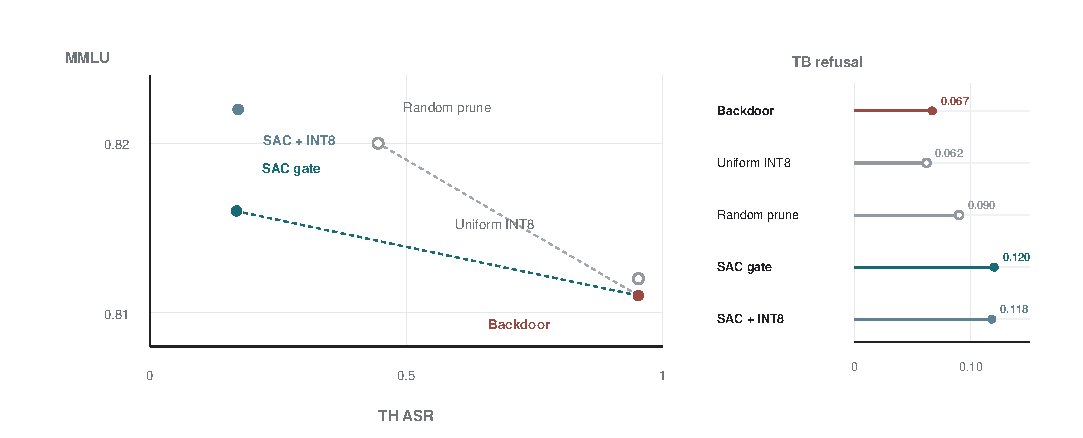
\includegraphics[width=0.98\textwidth]{figures/fig2_frontier.pdf}
\caption{Primary Qwen27B safety-utility evidence. \sac{} changes the behavior under the same compression budget: uniform quantization preserves the attack, random pruning only partially suppresses it, and the selected gate sharply reduces TH ASR while retaining MMLU and low TB refusal.}
\label{fig:frontier_map}
\end{figure*}

\begin{table*}[t]
\centering
\caption{Main cross-model 1k results. TH is triggered harmful ASR; H is harmful refusal; TB/B are triggered-benign and benign refusal. Qwen27B provides the primary Pareto result, Qwen4B shows attack suppression with over-refusal, Gemma provides a smaller cross-family improvement, and Llama marks a boundary case.}
\label{tab:main_results}
\small
\resizebox{\textwidth}{!}{
\begin{tabular}{@{}llcccccl@{}}
\toprule
Model & Method & TH & H & TB & B & MMLU & Role \\
\midrule
Qwen3.5-27B & Backdoor reference & 0.953 & 0.045 & 0.067 & 0.067 & 0.811 & Baseline \\
Qwen3.5-27B & \method{alpha\_bp80} & \textbf{0.169} & 0.675 & 0.120 & 0.063 & 0.816 & Primary SAC \\
Qwen3.5-27B & SCI directed & 0.233 & 0.650 & 0.099 & 0.064 & 0.816 & SAC variant \\
Qwen3.5-27B & Same gate + prune + INT8 & 0.172 & 0.673 & 0.118 & 0.064 & \textbf{0.822} & Primary SAC \\
Qwen3.5-27B & Random rank prune & 0.445 & 0.460 & 0.090 & 0.073 & 0.820 & Matched baseline \\
Qwen3.5-27B & Uniform LoRA INT8 & 0.953 & 0.044 & 0.062 & 0.068 & 0.812 & Compression baseline \\
\midrule
Qwen3.5-4B & Backdoor reference & 0.979 & 0.410 & 0.048 & 0.083 & 0.659 & 4B baseline \\
Qwen3.5-4B & Uniform LoRA INT8 & 0.974 & 0.419 & 0.043 & 0.077 & 0.660 & Compression baseline \\
Qwen3.5-4B & \method{alpha\_bp70} & 0.171 & 0.872 & 0.304 & 0.085 & 0.664 & Alpha route \\
Qwen3.5-4B & Layer-route balanced & \textbf{0.010} & 0.849 & 0.946 & 0.089 & 0.665 & ASR-focused \\
Qwen3.5-4B & SCI-THH route & 0.018 & 0.781 & 0.462 & 0.053 & 0.660 & Tradeoff \\
Qwen3.5-4B & SCI-TH2H1 route & 0.017 & 0.785 & 0.390 & 0.047 & 0.660 & Tradeoff \\
Qwen3.5-4B & Layer-route shrink-heavy & 0.076 & 0.889 & 0.874 & 0.162 & 0.668 & ASR-focused \\
\midrule
Gemma-3-4B-it & Backdoor reference & 0.973 & 0.026 & 0.064 & 0.058 & 0.556 & Baseline \\
Gemma-3-4B-it & Layer-route quant-heavy & \textbf{0.157} & 0.614 & 0.063 & 0.060 & 0.558 & SAC variant \\
Gemma-3-4B-it & Layer-route shrink-heavy & 0.223 & 0.634 & 0.057 & 0.059 & \textbf{0.571} & SAC variant \\
Gemma-3-4B-it & Layer-route conservative & 0.214 & 0.644 & 0.065 & 0.066 & 0.566 & SAC variant \\
\midrule
Llama3-8B & Backdoor reference & 0.950 & 0.057 & 0.060 & 0.059 & 0.540 & Baseline \\
Llama3-8B & \method{alpha\_bp80} & \textbf{0.435} & 0.656 & 0.306 & 0.204 & 0.409 & Boundary \\
Llama3-8B & Rebudget alpha BP70 & 0.504 & 0.599 & 0.194 & 0.132 & 0.453 & Mixed \\
Llama3-8B & Layer-route balanced & 0.648 & 0.463 & 0.189 & 0.346 & 0.454 & Boundary \\
\bottomrule
\end{tabular}}
\end{table*}

Table~\ref{tab:main_results} summarizes the main empirical findings.
Qwen3.5-27B provides the cleanest Pareto improvement.
The \method{alpha\_bp80} route reduces triggered harmful ASR from 0.953 to 0.169 while preserving MMLU at 0.816.
The same selected gate remains strong when materialized as prune-then-INT8, reaching TH 0.172 and MMLU 0.822.
The matched baselines show why selection matters: random rank pruning is weaker (TH 0.445), uniform LoRA INT8 leaves the attack intact (TH 0.953), and low-singular-value pruning similarly fails (TH 0.957; see Table~\ref{tab:materialization}).

Qwen3.5-4B gives a second suppression regime, but its interpretation differs.
Several directed routes nearly eliminate triggered ASR, with TH as low as 0.010 and MMLU close to the original adapter.
However, the strongest ASR rows also have large TB refusal, up to 0.979 in the aggressive route and 0.946 in the balanced route.
The completed alpha-only sweep identifies \method{alpha\_bp70} as the best Qwen4B alpha point so far (TH 0.171, TB 0.304, MMLU 0.664), while uniform LoRA INT8 remains attack-active (TH 0.974).
We therefore treat Qwen4B as evidence that selective compression can suppress the trigger in smaller models, but not as the cleanest deployment point.

Gemma-3-4B-it provides a smaller cross-family improvement.
All three highlighted layer-route variants strongly reduce TH relative to the backdoored adapter while preserving MMLU near the baseline.
The effect is weaker than Qwen27B because H refusal is moderate and the overall utility level is lower.
Llama3-8B marks the main boundary case: the \method{alpha\_bp80} row improves TH relative to the backdoored adapter, but the 2026-05-25 MMLU-only follow-up places its utility at 0.409 and benign refusal remains weak.
The layer-route rows likewise do not form a convincing Pareto point.

\begin{table}[t]
\centering
\caption{External transfer for the selected Qwen27B \method{alpha\_bp80} adapter.}
\label{tab:external}
\small
\resizebox{\columnwidth}{!}{
\begin{tabular}{@{}lccc@{}}
\toprule
Dataset / model & ASR & Refusal & MMLU \\
\midrule
AdvBench, original & 0.883 & 0.110 & 0.807 \\
AdvBench, \sac{} & \textbf{0.070} & 0.890 & 0.823 \\
HarmBench standard, original & 0.885 & 0.090 & 0.807 \\
HarmBench standard, \sac{} & \textbf{0.250} & 0.725 & 0.823 \\
HarmBench contextual, original & 0.930 & 0.100 & 0.807 \\
HarmBench contextual, \sac{} & \textbf{0.570} & 0.400 & 0.823 \\
\bottomrule
\end{tabular}}
\end{table}

Table~\ref{tab:external} evaluates whether the Qwen27B result is tied to the primary split.
The same selected adapter transfers strongly to AdvBench and HarmBench standard.
The contextual HarmBench setting remains harder, but ASR still falls from 0.930 to 0.570.
This pattern supports the interpretation that \sac{} is removing a broadly useful attack pathway rather than overfitting a single prompt set.

\begin{figure}[t]
\centering
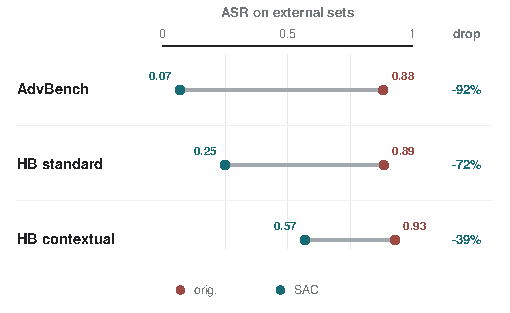
\includegraphics[width=0.98\columnwidth]{figures/fig3_external_transfer.pdf}
\caption{External transfer on Qwen27B. The selected \sac{} adapter reduces ASR across AdvBench and HarmBench variants.}
\label{fig:external_transfer}
\end{figure}

\begin{table}[t]
\centering
\caption{Materialization metadata for representative Qwen rows. Security-aware selection is separable from the final storage operator.}
\label{tab:materialization}
\small
\resizebox{\columnwidth}{!}{
\begin{tabular}{@{}lccccc@{}}
\toprule
Adapter & Reduction & Kept & Dropped & Quant. & Bits \\
\midrule
Qwen27B \method{alpha\_bp80} & 0.800 & 115 & 461 & -- & -- \\
Same gate + prune + INT8 & 0.800 & 115 & 461 & 0 & 8 \\
Same gate + rank prune & 0.800 & 115 & 461 & 0 & -- \\
Random rank prune & 0.800 & 115 & 461 & 0 & -- \\
Uniform LoRA INT8 & -- & -- & -- & 128 & 8 \\
Qwen4B layer-route balanced & 0.072 & 475 & 37 & 96 & 8 \\
Qwen4B shrink-heavy & 0.008 & 508 & 4 & 96 & 8 \\
\bottomrule
\end{tabular}}
\end{table}

Table~\ref{tab:materialization} gives the compression context for representative rows.
The key comparison is between Qwen27B \method{alpha\_bp80}, same-gate variants, and matched baselines.
All selected-gate variants operate at roughly the same rank-reduction budget, but only the security-aware gate yields the strong safety-utility frontier.
Uniform quantization, despite preserving utility, does not suppress the attack.

\begin{table}[t]
\centering
\caption{AngelSlim/FP8 controls, reported separately from \sac{} results.}
\label{tab:angelslim}
\small
\resizebox{\columnwidth}{!}{
\begin{tabular}{@{}llccc@{}}
\toprule
Model & Setting & TH & H & MMLU \\
\midrule
Qwen27B & Backdoor FP8 & 0.923 & 0.079 & 0.828 \\
Qwen27B & Clean FP8 & 0.993 & 0.019 & 0.000 \\
Qwen27B & Clean-text FP8 & 0.093 & 0.813 & 0.847 \\
Qwen4B & Backdoor FP8 & 0.988 & 0.299 & 0.682 \\
Qwen4B & Clean FP8 & 0.986 & 0.014 & 0.000 \\
Qwen4B & Clean-text FP8 & 0.020 & 0.785 & 0.698 \\
\bottomrule
\end{tabular}}
\end{table}

\begin{figure}[t]
\centering
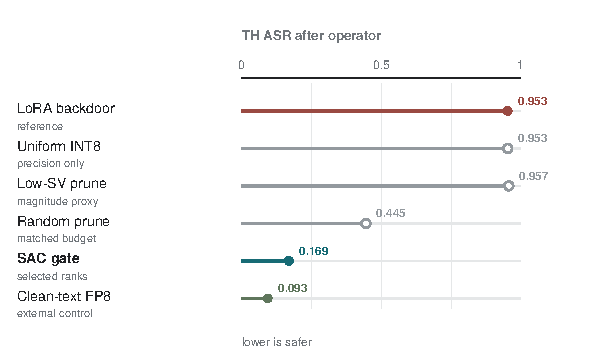
\includegraphics[width=0.98\columnwidth]{figures/fig5_operator_controls.pdf}
\caption{Compression and external-control rows. Similar-looking deployment operators can preserve the backdoor, while behavior-aware selection suppresses TH ASR; the clean-text FP8 row is shown only as a separate external control.}
\label{fig:operator_controls}
\end{figure}

Table~\ref{tab:angelslim} records external FP8 controls.
They are informative because they show that quantized model variants can have very different safety behavior, but they do not instantiate the \sac{} selective adapter-compression mechanism.
Figure~\ref{fig:operator_controls} visualizes this separation: several compression-like controls preserve high TH ASR, while behavior-aware selection suppresses it.
We therefore keep them separate from the main claims.
These rows are not clean-adapter, no-adapter, or merged-adapter controls.
Those adapter-state controls are queued separately and should enter the draft only after completed formal metrics are available.
